From the given information,
\begin{enumerate}
\item 
\begin{align}
\pr{X>9000} &= \frac{325 +445}{1000}
\\
&=0.77
\end{align}
\item 
\begin{align}
\pr{4000<X<14000} &= \frac{20+210+325}{1000}
\\
&=0.0.555
\end{align}
\item 
\begin{align}
\pr{X<4000} &= \frac{20}{1000}
\\
&=0.02
\end{align}
Related codes are available in 
\begin{lstlisting}
solutions/1-10/codes/probexm/probexm6.py
\end{lstlisting}
%\begin{figure}[!ht]
%	\centering
%	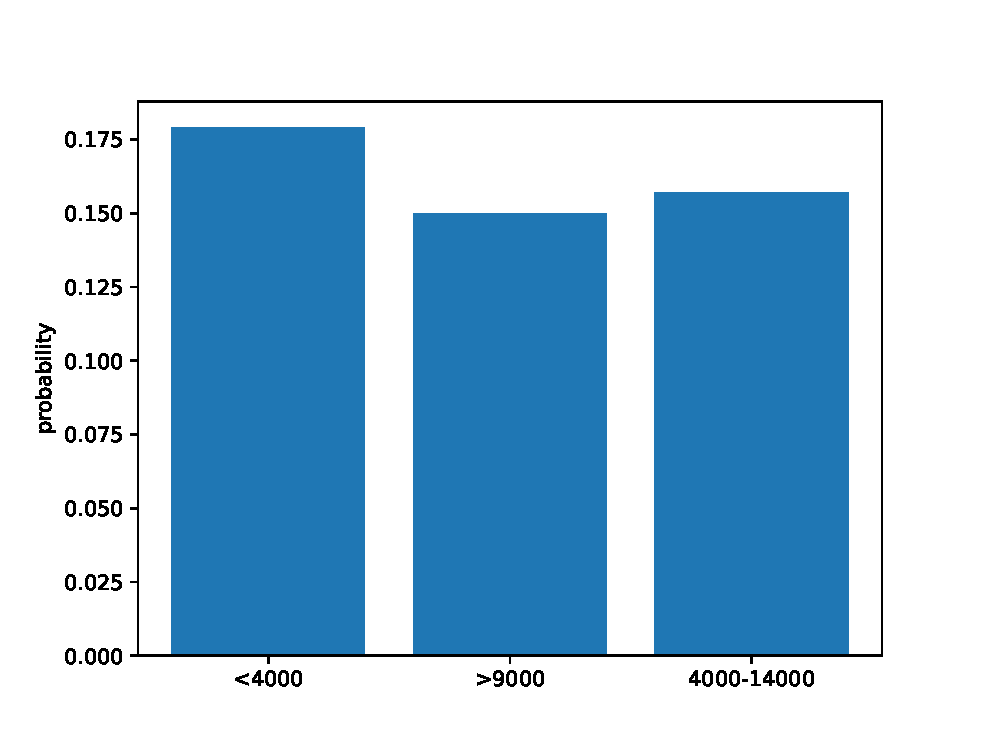
\includegraphics[width=\columnwidth]{./figures/probexm/probexm6.eps}
%	\caption{probability of distance covered by tyre }
%	\label{fig:bt6}
%	\begin{lstlisting}
%	figs/probexm/probexm6.eps
%	\end{lstlisting}
%\end{figure}
\end{enumerate}
